\documentclass[oneside,9pt]{article}
\usepackage[a4paper,width=170mm,top=18mm,bottom=22mm,includeheadfoot]{geometry}
\pdfoutput=1
\usepackage{multicol}
\usepackage{amsmath}
\usepackage{amssymb}
\usepackage{caption}
\usepackage{hyperref}
\usepackage{mathtools}
\usepackage[linesnumbered,algoruled,boxed,lined]{algorithm2e}
\usepackage{graphicx}
\usepackage{float}

\hypersetup{
    colorlinks=true,
    urlcolor=cyan
}
\hypersetup{final}

% paper version
\newcommand{\PaperVersionNumber}{0.1 - 2018-02-28}

\providecommand{\keywords}[1]{\textbf{\textit{Keywords---}} #1}

% list of elements
\newcommand{\lista}[3][_]{ #2#10, \dots, #2#1{#3} }
% set
\newcommand{\setd}[1]{ \mathit{#1} }
\newcommand{\setl}[2]{ \left\{ \lista{#1}{#2} \right\}  }
% vector
\newcommand{\vecd}[1]{ \textbf{#1} }
\newcommand{\vecl}[2]{ (\lista{#1}{#2}) }
% poly
\newcommand{\poly}[2]{ p_{\textbf{#1}}(#2) }
\newcommand{\polysum}[3][x]{ #2_0 + #2_1 #1 + #2_2 #1^2 + \dots + #2_{#3} #1^{#3} }
% big O
\newcommand{\bigo}[1]{ \mathcal{O}(#1) }

% evaluated point
\newcommand{\ele}{s}
% linear codes \ec{n}{k}
\newcommand{\ec}[2]{ \mathcal{C}(#1, #2) }
% finite field \gf{q} or \gf[n]{p}
\newcommand{\gf}[2][]{ \mathbb{F}_{{#2}^{#1}} }
% ring nf4
\newcommand{\ringn}[1][n]{ \mathbb{R}_{F_4}(#1) }
% fft
\newcommand{\fft}[1]{ \text{FFT}(#1) }
\newcommand{\fftl}{N}
% coef
\newcommand{\ith}[1]{#1^\text{th}}
% set of points
\newcommand{\sete}{\setd{S}}
% complexity
\newcommand{\an}[1][N]{\mathcal{A}(#1)}
\newcommand{\mn}[1][N]{\mathcal{M}(#1)}
% F4
\newcommand{\ffour}{65537}
\newcommand{\ffourMinusOne}{65536}
% operator
\newcommand{\op}{\diamond}

\DeclarePairedDelimiter{\ceil}{\lceil}{\rceil}
\newcommand*\eg{e.g.\@\xspace}
\newcommand*\Eg{e.g.\@\xspace}
\newcommand*\ie{i.e.\@\xspace}
\newcommand*\samethanks[1][\value{footnote}]{\footnotemark[#1]}

%\renewcommand{\itemhook}{\setlength{\topsep}{0pt}  \setlength{\itemsep}{0pt}\setlength{\leftmargin}{15pt}}

%% Authors
\author{ Vianney Rancurel\thanks{Scality in San Francisco, CA, 94104.}\\ \texttt{vianney.rancurel@scality.com}
    \and L\^am Pham-Sy\thanks{Scality France.}\\ \texttt{lam.pham-sy@scality.com} 
    \and Sylvain Laperche\samethanks[3]\\ \texttt{sylvain.laperche@scality.com}
}

\title{QuadIron: A library for Number Theoretic Transform-based Erasure Codes\thanks{Manuscript received Januray 12, 2020.}}

\begin{document}
\maketitle

\begin{abstract}
Reed-Solomon codes can be seen as polynomial operations which can be implemented by number theoretic transforms and accelerated by different fast Fourier transform algorithms according to the characteristics of the fields. We present a library, QuadIron, which implements FFTs in binary, prime, and extension fields, as well as a set of optimizations to make them practical for a very large number of symbols. These FFT-based erasure codes could be useful for applications like decentralized storage over Internet, or real-time video high-quality streams.
\end{abstract}


\keywords{Number Theoretic Transforms, Discrete Fourier Transforms, Finite Fields, Erasure Codes, Digital Storage, Distributed storage, Decentralized Storage, Decentralized Cloud Storage, Real-time video, high-quality streaming}


\section{Introduction}
\label{sec:introduction}

A {$\ec{n}{k}$} erasure code is defined by $n=k+m$, $k$ being the number of data fragments, $m$ being the number of desired erasure fragments. In an application it is required to transmit the $n$ fragments. A Maximum Distance Separable (MDS) code guarantees that any $k$ fragments can be used to decode a file. Erasure codes can be either systematic or non-systematic. Systematic codes generate $n-k$ erasure fragments and therefore maintain $k$ data fragments. Non-systematic codes generate $n$ erasure fragments. In the case of systematic codes, we try to retrieve primarily the $k$ data fragments if possible because there is nothing to decode. A decoding is necessary only if one or more data fragments are missing. In the case of non-systematic codes, we need to decode $k$ fragments. Erasure codes can also be compared by their sensitivity to the rate $r=k/n$, which may or may not impact the encoding and decoding speed. Another comparison criterion is the support of adaptive rate: does the erasure code allows to change $k$ and $m$ dynamically, without having to regenerate the whole set of erasure fragments. Another critical property is called the 'confidentiality' \cite{li_confidentiality} which is determined if an attacker can partially decode the data if he obtains less than k fragments. Finally, we can also compare erasure code according to their repair bandwidth, i.e.\ the number of fragments required to repair a fragment. To sum up, here is a list of codes' properties that are of interest for us:
\begin{itemize}
\item MDS/non-MDS
\item Systematic/Non-systematic
\item Encoding/Decoding speed according to various $n$
\item Encoding/Decoding speed predictivity and stability acc/ to $n$
\item Rate sensitivity
\item Adaptive vs non-adaptive rate
\item Confidentiality
\item Repair bandwidth
\end{itemize}

Reed-Solomon (RS) codes are MDS codes constructed from Vandermonde or Cauchy matrices \cite{reed_sol} that are systematic and support adaptive rates. The RS encoding process is traditionally performed by multiplying a $[n \times k]$ matrix by a $k$ data vector in $\gf{2^w}$, leading to a high complexity of $\bigo{k \times n}$. The topic of optimizing those codes has been widely discussed. While such optimizations reduce the overall complexity, most of them rely solely on hardware optimizations, therefore their real complexity in ''big O'' notation has not been widely studied.
% * <wabernat@sonic.net> 2018-03-02T18:03:30.509Z:
% 
% Question on notation: I am assuming that an n*k matrix is a different expression than k x n. If not, make them the same.
% 
% ^.

Low-Density-Parity-Check (LDPC) codes are also an important class of erasure codes and are constructed over sparse parity-check matrices. Although initially used in networking applications, some researchers recently showed that it is possible to use them in distributed storage scenarios \cite{plank_ldpc}. Those codes, which even though require to store $n=k+m$ fragments (like MDS codes), need to retrieve $[f \times k]$ fragments to recover the data (instead of only $k$ for MDS codes), $f$ being called the overhead or the inefficiency. The study \cite{plank_ldpc} shows 3 types of LDPC codes where $f$ oscillates between $1.10$ and $1.30$ for $n \lessapprox 100$, and shows that you need a larger $n$, e.g.\ $n \gtrapprox 1000$ in order to have an $f$ approaching $1.0$. As shown by \cite{plank_ldpc}, those codes are more sensible to network latency because of the extra fragments, due to the overhead, that they need to retrieve, so in cases where latency can be important RS codes seems more interesting than LDPC codes. More recently hybrid-LDPC schemes such as \cite{wirehair} have reduced the overhead to $[k + f]$ with a very small f. Also, \cite{park_ldpc} have shown that it is possible to design LDPC codes which beat RS codes when taking into account the repair bandwidth, because RS codes always need to retrieve $k$ fragments to be able to repair the data, while it is possible to design LDPC codes that require less than $k$ fragments for the repair process. However:
\begin{itemize}
\item LDPC are not MDS: it is always possible to find a pattern (e.g.\ stopping sets) that cannot decode (e.g. having only k fragments out of n).
\item You can always find/design an LDPC code optimized for few properties (i.e.\ tailored for a specific use case) that beats other codes on those few properties, but there is no silver bullet: it will be sub-optimal for the other properties (its a trade-off, e.g.\ good for large $n$ and with an optimal repair bandwidth, but not good for small $n$ and cannot support adaptive rate): these cannot be used in a generic library.
\item Designing a good LDPC code is some kind of black art that requires a lot of fine tuning and experimentation. Ultimately an LDPC code optimal for all the interesting properties for a given use case could exist but would be very complex and/or would only be available in a commercial library.
\end{itemize}

Recently some other types of codes, called Locally-Repairable-Codes (LRC) \cite{xor_elephant} \cite{erasure_azure}, have tackled the repair bandwidth issue of the RS codes. They combine multiple layers of RS: the local codes and the global codes. However those codes are not MDS and they require an higher storage overhead than MDS codes.

Fast Fourier transform (FFT) based RS codes remain relatively simple, and can be used to perform encoding on finite fields with clearer and lower announced complexities therefore having a good set of desirable properties:
\begin{itemize}
\item They are MDS
\item Support both systematic or non-systematic codes
\item Fast for a wide range of $n$
\item Rate insensitive (for non-systematic codes).
\item Confidential (for systematic codes).
\end{itemize}
We focus our research on optimizing their encoding and decoding speed.
% * <wabernat@sonic.net> 2018-03-02T18:07:38.602Z:
% 
% > Recently, thanks to fast Fourier transform
% Are you announcing your findings here? If so: "We have found that using FFT..."
% 
% ^.

Since the computational complexities of FFT operations mainly depend on the chosen finite field, we investigate two types of finite fields: prime finite fields and binary extension finite fields. For each type, there are different approaches to accelerate the FFT operations.

%\hfill The authors
 
%\hfill April 26, 2018

\section{Reed-Solomon codes}
%%%%%%%%%%%%%%%%%%%%%%%%

A Reed-Solomon (RS) code is an MDS code $\ec{n}{k}$ defined over a finite field $\gf{q}$ where $q$ is a prime power $q=p^w$. A code word composed of $n$ symbols is generated from a message of length $k$. The message is recovered from a subset of at least $k$ elements of the code word.
% * <wabernat@sonic.net> 2018-03-02T18:23:50.138Z:
% 
% > code word
% Changing this to code word from "codeword" globally. If you know better (i.e., if "codeword" is a widely accepted neologism), you can roll it back.
% 
% ^.

\subsection{Encoding}
As  Reed and Solomon described in their foundational paper\cite{reed_sol}, a code word is encoded from a message using polynomial evaluation. 

A message $\vecd{m} = \vecl{m}{k} \in \gf{q}^k$ can be represented as a polynomial $\poly{m}{x}$ of degree $k-1$:

\begin{equation}\label{eq:poly}  
	\poly{m}{x} = \polysum{m}{k-1}
\end{equation}

The code word $\vecd{c} = \vecl{c}{n-1}  \in \gf{q}^n$ of the message $\vecd{m}$ is obtained by evaluating $\poly{m}{x}$ at a given but arbitrary set of $n$ \emph different points $\sete = \setl{\ele}{n-1}$ of the field $\gf{q}$,  called the set of evaluation points. Concretely,

\begin{equation}\label{eq:enc_def}
\begin{split}
	c_0 &= \polysum[\ele_0]{m}{k-1},\\
	c_1 &= \polysum[\ele_1]{m}{k-1},\\
	& \dots \\
	c_{n-1} &= \polysum[\ele_{n-1}]{m}{k-1}\\
\end{split}
\end{equation}

Equation (\ref{eq:enc_def}) can be represented as a multiplication of the message $\vecd{m}$ and matrix $G$:

\begin{equation}
\vecd{c} = \vecd{m} \times G
\end{equation}
 where $G$ is the generator matrix of the RS codes:

\begin{equation}\label{eq:gen_mat}
G = \begin{bmatrix}
1 & 1 & \dots & 1 \\
\ele_0 & \ele_1 & \dots & \ele_{n-1} \\
\ele_0^2 & \ele_1^2 & \dots & \ele_{n-1}^2 \\
\vdots & \vdots & & \vdots \\
\ele_0^{k-1} & \ele_1^{k-1} & \dots & \ele_{n-1} ^{k-1}
\end{bmatrix}
\end{equation}

Since $\ele_i \neq \ele_j$ when  $i \neq j$, $G$ is actually a Vandermonde matrix \cite{book_ecc}.
% * <wabernat@sonic.net> 2018-03-02T18:31:07.849Z:
% 
% > for
% do you mean "when" or "because"?
% 
% ^.

Straightforwardly, the encoding process has a computational complexity of $\bigo{k \times n}$ for performing a multiplication of a vector $\vecd{m}$ and a matrix $G$.

This complexity can be reduced by using a Discrete Fourier Transform (DFT) on a finite field that evaluates polynomial $\poly{m}{x}$ at the set $\sete$ of evaluating points. Currently, two main Fast Fourier Transform (FFT) techniques apply for prime field $\gf{p}$ \cite{cooley_tukey,fnt_lacan,fnt_ida}, and for binary extension field $\gf{2^w}$ \cite{fft_add_wang_zhu,fft_add_cantor,fft_add_gao_mateer,fft_add_chung}. We summarize these techniques in Section \ref{sec:fft}. Briefly, thanks to the FFT techniques, the encoding complexity drops to $\bigo{n \times \log{n}}$.

%Briefly, the codeword $\vecd{c}$ can be calculated by one FFT operation on message $\vecd{m}$:
%\begin{equation}\label{eq:fft_1}
%\vecd{c} = \fft{\vecd{m}}
%\end{equation}

\subsection{Decoding}

A message $\vecd{m}$ can be decoded from a code word $\vecd{c}$ that could miss at most $n-k$ elements. Indeed, given a set of $k$ coefficients of $\vecd{c}$, the polynomial $\poly{m}{x}$ in Equation (\ref{eq:poly}) can be regenerated using Lagrange interpolation because its degree is at most $k-1$. Let $\setl{\tilde{c}}{k-1}$ denote the set of $k$ known coefficients corresponding to $k$ evaluation points $\setl{\tilde{\ele}}{k-1}$. The polynomial $\poly{m}{x}$ is thus interpolated:

\begin{equation}
\label{eq:lagrange}
\poly{m}{x} = \sum_{i=0}^{k-1} \big( \tilde{c}_i \times \sum_{0 \leq j \leq k-1, j \neq i} \frac{x - \tilde{\ele}_j}{ \tilde{\ele}_i - \tilde{\ele}_j } \big)
\end{equation}

Coefficients of the message $\vecd{m}$ are actually coefficients of $\poly{m}{x}$.

On prime field, equation \ref{eq:lagrange} can be simplified as proposed in \cite{fnt_lacan}. Note that degree of $\poly{m}{x}$ is at most $(k-1)$, the polynomial is derived as:

\begin{equation}
\poly{m}{x} =  \Big( A(x) \times \sum_{i=0}^{k-1} \frac{n_i}{x -  \tilde{\ele}_i}  \Big) \text{ mod } x^k
\end{equation}
where
\[
\begin{split}
A(x) &= \prod_{i=0}^{k-1}(x -  \tilde{\ele}_i), \\
n_i &= \frac{ \tilde{c}_i }{ A'( \tilde{\ele}_i) }
\end{split}
\]

Using Taylor series, we have

\[
\frac{1}{ \tilde{\ele}_i - x } = \sum_j \frac{ x^j }{ {\tilde{\ele}_i}^{j+1} }
\]

And by defining the following polynomial:
\[
N(x) := \sum_{i = 0}^{k-1} \frac{n_i}{\tilde{\ele}_i} \times x^{z_i}
\]
where its exponents $\{z_i, i = 0, \dots, k-1 \}$ are determined by the evaluation set $S$ and the $\ith{n}$-root of unity $r$
\[
\tilde{\ele}_i = r^{z_i}, \ i = 0, \dots, k-1
\]
 
 We obtain a simpler formula:

\begin{equation}
\poly{m}{x} =  \Big( A(x) \times B(x) \Big) \text{ mod } x^k
\end{equation}
where $B(x) := \sum_{i=0}^{k-1} N(r^{-i}) x^i $ whose coefficients are obtained by evaluating $N(x)$ at $k$ points $\{ r^{-i} \}$ that can be efficiently performed using the inverse FFT algorithm.

Thanks to the convolution theorem, we can use FFT techniques to accelerate the multiplication of two polynomials $A(x), B(x)$:
\begin{equation}
A(x) \times B(x) = iFFT_{2k} ( FFT_{2k}(A) \cdot FFT_{2k}(B) )
\end{equation}
where $FFT_{2k},  iFFT_{2k}$ are FFT and inverse FFT of length $2 \times k$.

Note that $A(x)$ depends only on evaluation points, hence $A(x), A'(x), FFT_{2k}(A)$ can be calculated once.

The decoding computation is composed of:
(1) one inverse FFT of length $n$ to compute $N(x)$;
(2) one FFT and one inverse FFT of length $2k$ to compute $A(x) \times B(x)$.
It leads to a decoding complexity of $\bigo{ n \log n + 4 k \log{2k}}$.

Compared to \cite{fnt_lacan}, our computations are based on the fact that the degree of $\poly{m}{x}$ is smaller than $k$. Hence we use $2k$-length FFT instead of $2n$-length FFT.

%%%%%%%%%  Section %%%%%%%%%%
\section{How can FFT reduce Encoding Complexity?}\label{sec:fft}
%%%%%%%%%%%%%%%%%%%%%%%%

In this section, we summarize two FFT techniques on the field $\gf{q}$ that can the reduce computational complexity of the encoding process. Their common methodology is to split an FFT operation on a vector $\vecd{m}$ into two FFT operations on a smaller set $\vecd{m}_1$ and $\vecd{m}_2$. 
Let $\fftl$ denote the length of input vector $\vecd{m}$ that is also represented as a polynomial $\poly{m}{x}$

\begin{equation}\label{eq:poly_fft}  
	\poly{m}{x} = \polysum{m}{\fftl-1}
\end{equation}

Given a set $\sete = \setl{\ele}{\fftl-1}$ of different elements of $\gf{q}$, FFT transforms the input vector to an output vector $\vecd{c}$ whose coefficients are values of $\poly{m}{x}$ evaluated at points of $\sete$.

\begin{equation}\label{eq:enc_fft}  
	\vecd{c} = \big( \poly{m}{\ele_0}, \poly{m}{\ele_1}, \dots, \poly{m}{\ele_{\fftl-1}} \big)
\end{equation}

This is similar to the described RS encoding process, except that the input and output vectors are of the same length $\fftl$.

The key factor that allows splitting FFTs into smaller transformations is choosing the set $\sete$. The two methods of constructing such a set are described here.
% * <wabernat@sonic.net> 2018-03-02T18:43:34.525Z:
% 
% > The key factor that allows splitting FFT into smaller ones is choosing the set $\sete$.
% Smaller whats? 
% 
% ^.

\subsection{$\sete$ as multiplicative group}

The set $\sete$ is constructed as a multiplicative group whose generator is the $\ith{\fftl}$ root of unity of the field $\gf{q}$, i.e.

\begin{equation}
\sete = \left\{ \lista[^]{\alpha}{\fftl-1} \right\}
\end{equation}
where $\alpha$ is the $\ith{\fftl}$ root of unity of the field $\gf{q}$. We call this technique \textit{multiplicative FFT}.

The FFT technique applied for the constructed set $\sete$ was first introduced in \cite{cooley_tukey}. Supposing that $\fftl = \fftl_1 \times \fftl_2$, the FFT operation on $\vecd{m}$ is split into two FFT operations on two vectors $\vecd{m}_1$ and $\vecd{m}_2$ of length $\fftl_1$ and $\fftl_2$ respectively. This results in a computational complexity $\bigo{\fftl(\fftl_1+\fftl_2)}$. If $\fftl$ is highly composite, this technique reduces the computation time to $\bigo{\fftl\log{\fftl}}$.

To obtain such advantages, however, this technique requires the satisfaction of two conditions:
\begin{enumerate}
\item $\fftl$ is a divisor of $q-1$ (for the existing $\ith{\fftl}$ root of unity of the field $\gf{q}$),
\item $\fftl$ is highly composite, e.g. $\fftl = 2^v$ ideally
\end{enumerate}

A simple solution to satisfying these conditions  is to use the field $\gf{q=p^w}$ where  $p$ is prime and $p-1$ is highly composite. Fermat numbers, i.e. $F_i = 2^{2^i} + 1$ for $i \leq 4$, are perfectly suitable for that. This technique, also called Fermat Number Transform (FNT) based erasure codes, was introduced and analyzed in \cite{fnt_lacan, fnt_ida}.

This technique, however, does not efficiently apply to the binary extension field $\gf[w]{2}$ because divisors of $(2^w-1)$ are not highly composite. However, $\gf[w]{2}$ is perfectly suitable for most practical applications because each element can be expressed by $n$ bits. The following FFT technique focuses on this field.

\subsection{$\sete$ as additive group}

This technique focuses on the binary extension field $\gf[w]{2}$. Introduced in\cite{fft_add_wang_zhu, fft_add_cantor}, it was recently improved in \cite{fft_add_gao_mateer} by using Taylor extension algorithms. A further improvement is shown in \cite{fft_add_chung}.

%We describe briefly the technique introduced in \cite{fft_add_gao_mateer}. 
The FFT length is necessarily a power of 2, i.e. $\fftl = 2^m$ with $m \leq w$.
Let $\lista{\beta}{m-1}$ be $m$ linearly independent elements of $\gf[n]{2}$. The set $\sete$ is chosen as a subspace spanned by $\beta_i$ over $\gf{2}$, i.e.

\begin{equation}
\begin{split}
\ele_i = i_0 \beta_0 + i_1 \beta_1 + i_2 \beta_2 + \dots + i_{m-1} \beta_{m-1},\\
\text{ for } 0 \leq i \leq 2^m-1\\
\end{split}
\end{equation}

where $i = \polysum[2]{i}{m-1}$ with $i_j \in \gf{2}$.
The FFT operation on a vector $\vecd{m}$ is re-expressed as two FFTs on two vectors of half length.

\subsection{Computational complexity}

Let $\an[\fftl]$ denote the number of additions or subtractions in the field $\gf{q}$ needed for an FFT operation with an input vector of length $\fftl$  (assuming that an addition requires the same amount of effort to implement as a subtraction).

Let $\mn[\fftl]$ denote the number of multiplications required in the field $\gf{q}$ needed for an FFT operation with an input vector of length $\fftl$.

The computational complexities of these algorithms are shown in Table \ref{tab:compare}, which shows that, with suitable parametrization of the FFT length and the field $\gf{q}$, multiplicative FFT is faster than all available additive FFTs.

\begin{table*}[!ht]
 \caption{Computational complexity of FFT techniques}
 \label{tab:compare}
 \begin{center}
 \begin{tabular}{|c | c | c | c|} 
 \hline
 Name
 	& Restriction
	& Addition $\an[\fftl]$
	& Multiplication $\mn[\fftl]$
	\\ \hline
 Multiplicative FFT 
 	& $\fftl = 2^v$ and $(q-1) \% \fftl = 0$ 
 	& $\fftl \log_2(\fftl)$  
	& $\frac{1}{2} \fftl \log_2(\fftl) - \fftl + 1$
	\\ \hline
 Additive FFT \cite{fft_add_gao_mateer}
 	& $\fftl = 2^v$ and $q=2^w$
	& $4 \fftl (\log_2(\fftl))^2 + \frac{3}{4} \fftl \log_2(\fftl) - \frac{1}{2} \fftl$ 
	& $2 \fftl \log_2(\fftl) - 2 \fftl + 1$
	\\ \hline 
 Additive FFT \cite{fft_add_gao_mateer}
 	& $\fftl = 2^{2^v}$ and $q=2^w$
	& $\fftl \log_2(\fftl) + \frac{1}{2} \fftl \log_2(\fftl) \log_2\log_2(\fftl)$ 
	& $\frac{1}{2} \fftl \log_2(\fftl)$
	\\ \hline 
 Additive FFT \cite{fft_add_chung}
 	& $\fftl = 2^{v}$ and $q=2^w$
	& $\fftl \log_2(\fftl) $ 
	& $\frac{1}{2} \fftl \log_2(\fftl)$
	\\ \hline 
 \end{tabular}
 \end{center}
\end{table*}

%%%%%%%%%  Section %%%%%%%%%%
\section{The QuadIron library}
%%%%%%%%%%%%%%%%%%%%%%%%

The QuadIron library is a C++ library, written in C++14, that provides a streaming API to use the different flavors of NTT-based erasure codes.

The library focuses primarily on high fragmentation, i.e. $n \gg k$.

It includes general modular arithmetic routines, algorithms for manipulating rings of integers modulo \textit{n}, finite fields (including binary, prime, and non-binary extension fields), polynomial operations, different flavors of discrete Fourier transforms, and forward error correction (FEC) algorithms.
% * <wabernat@sonic.net> 2018-03-02T19:25:31.132Z:
% 
% >  (non-binary)
% Parens why?
% 
% ^.
% * <wabernat@sonic.net> 2018-03-02T19:24:18.536Z:
% 
% > n
% italic?
% 
% ^.

The library also includes an abstraction for writing systematic and non-systematic codes, although for applications requiring high fragmentation, systematic codes are not especially useful.

\subsection{Optimizations}

The QuadIron library's code relies heavily on templates to generate specifically optimized code at compile time. We use this template to allow a selection of numeric types matching the size of the processor's registers to optimize performance.

\subsection{Vectorization} \label{sec:vectorization}

We focus here on vectorizing multiplicative FFTs which are based on prime (non-binary) field $\gf{q}$ operations.

We observe that there are three operations that are costly in multiplicative FFT transformation: addition, subtraction and Hadamard multiplication. All of them are element-wise operations where the inputs are two vectors $\vec{a}, \vec{b}$ and the output is a vector $\vec{c}$. All of these vectors are of the same length $n$.

\begin{equation}
\begin{split}
\vec{a} = (a_1, a_2, \dots, a_n) \\
\vec{b} = (b_1, b_2, \dots, b_n) \\
\vec{c} = (c_1, c_2, \dots, c_n)
\end{split}
\end{equation}

\begin{itemize}
\item Addition
$$
c_i = (a_i + b_i) \% q, \text{ for } i = 1, \dots, n
$$
\item Subtraction
$$
c_i = (a_i - b_i) \% q, \text{ for } i = 1, \dots, n
$$

\item Hadamard multiplication
$$
c_i = (a_i * b_i) \% q, \text{ for } i = 1, \dots, n
$$

\end{itemize}

For simplicity, we express these operations by using a super-operator $\oplus$ as below:

\begin{figure}[H]
\centering
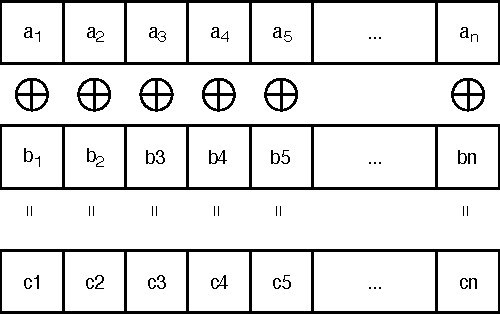
\includegraphics[width=0.5\columnwidth]{operator.pdf}
\caption{Element-wise operations $\vec{c} = \vec{a} \oplus \vec{b}$}
\label{fig:operator}
\end{figure}

We accelerate these operations in two ways: horizontal and vertical vectorizations. Note that the number of operations performed in parallel depends on bit-size of the elements and the bit-size of the vector registers. For example, if elements are 32-bit integers and registers are 128-bit wide, then there are 128/32 = 4 operations that can be performed in parallel.

Without loss of generality, we assume that 4 element-wise operations can be performed in parallel.

\subsubsection{Horizontal vectorization}

Each vector is defined as an $n$-length array of integers. Four operations applied on four consecutive elements of $\vec{a}$ and $\vec{b}$ are performed in parallel. Therefore,  operations on $\vec{a}$ and $\vec{b}$ corresponds to $\frac{n}{4}$ vector operations.

\begin{figure}[!ht]
\centering
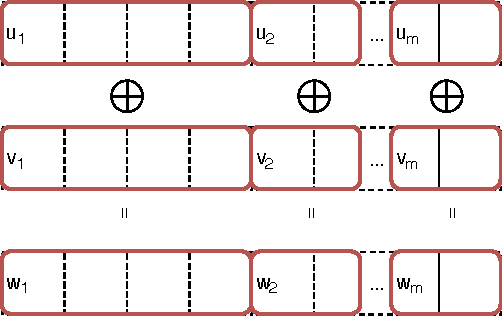
\includegraphics[width=0.5\columnwidth]{vec_horizontal.pdf}
\caption{Horizontal vectorization}
\label{fig:vec_horizontal}
\end{figure}


\subsubsection{Vertical vectorization}

\begin{figure}[!ht]
\centering
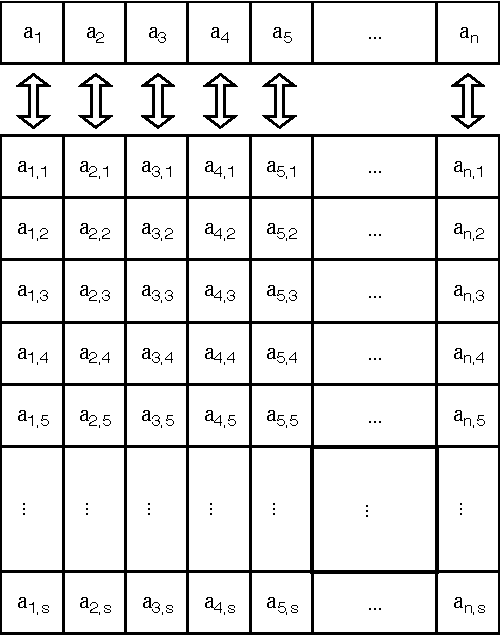
\includegraphics[width=0.5\columnwidth]{vec_buffers.pdf}
\caption{Vector of buffers}
\label{fig:vec_buffers}
\end{figure}

\begin{figure*}[!ht]
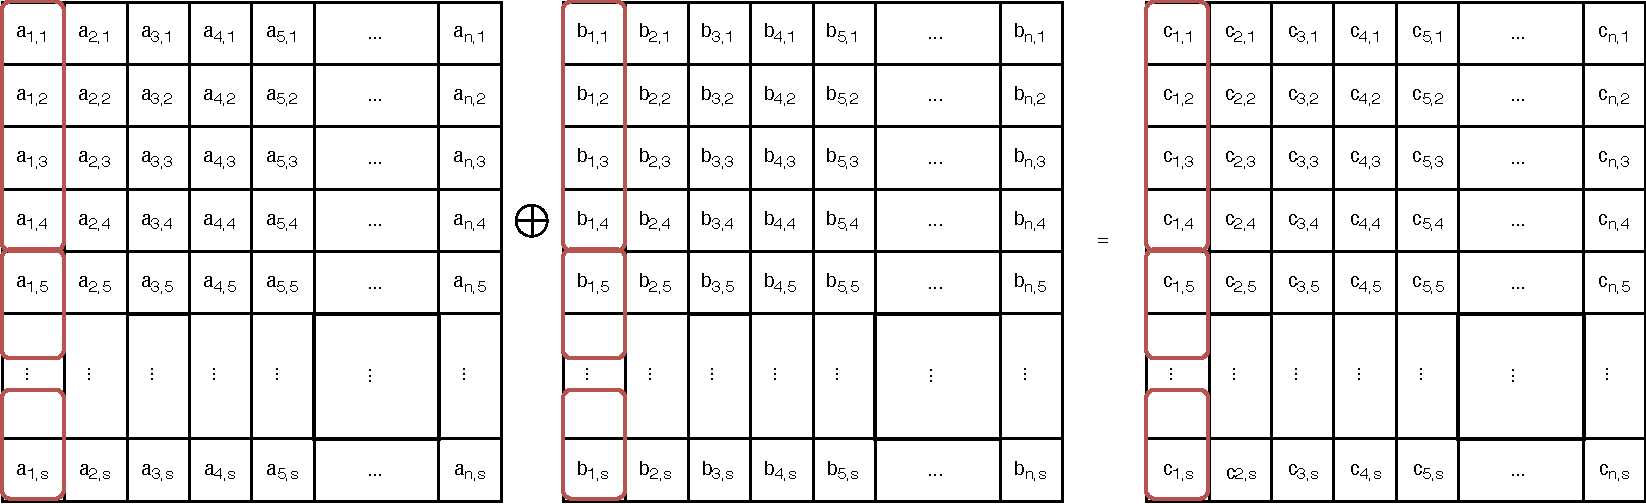
\includegraphics[width=\textwidth]{vec_vertical.pdf}
\caption{Vertical vectorization}
\label{fig:vec_vertical}
\end{figure*}

Each vector is defined as an $n$-length array of buffers. Each element of these vectors is a buffer composed of  integers, see Figure \ref{fig:vec_buffers}.

An operation $c_i = a_i \oplus b_i$ is equivalent to $s$ operations performed on $s$ elements each of $a_i$ and $b_i$. 
We accelerate operations performed on each pair of buffers $a_i$ and $b_i$,  i.e.\ in vertical way as shown in Figure \ref{fig:vec_vertical}. Four operations applied on four consecutive elements of $a_i$ and $b_i$ are performed in parallel. Therefore, $s$ operations on $a_i$ and $b_i$ corresponds to $\frac{s}{4}$ vector operations.

\subsection{Vectorized modular operations in $\gf{q}$ where $q$ is a Fermat number}

In the previous section, we described the two methods to transform element-wise operations to packed vector operations. Each vector operation performs several element-wise operations in parallel. In this section, we describe how the parallel operations are performed on packed vectors.

Note that we focus on vectorizing modular arithmetic of finite field $\gf{q}$ where $q=2^{2^w}+1$, a Fermat number.
This case is very interesting since it allows performing multiplicative FFT of low computational complexity (see the 1st row of Table \ref{tab:compare}) \cite{fnt_lacan}

Let $\vec{q}$ denote a packed vector whose elements are $q$.
Let $\vec{h}$ denote a packed vector whose elements are $q-1$.
Let $\vec{u}, \vec{v}$ denote two input packed vectors. 

Let $vector_<operation>(\vec{u}, \vec{v})$ denote an instruction that applies an operation on two input packed vectors $\vec{u}, \vec{v}$.

\begin{itemize}
\item \texttt{vector\_add}$(\vec{u}, \vec{v})$ does element-wise addition
\item \texttt{vector\_sub}$(\vec{u}, \vec{v})$ does element-wise subtraction
\item \texttt{vector\_mullo}$(\vec{u}, \vec{v})$ does element-wise multiplication
\item \texttt{vector\_or}$(\vec{u}, \vec{v})$ compute bitwise OR operation
\item \texttt{vector\_and}$(\vec{u}, \vec{v})$ compute bitwise AND operation
\item \texttt{vector\_andnot}$(\vec{u}, \vec{v})$ compute bitwise NOT of $\vec{u}$ then AND with $\vec{v}$
\item \texttt{vector\_cmpgt}$(\vec{u}, \vec{v})$ returns $((u_i > v_i) ? 1 : 0, i=1, \dots, n)$
\item \texttt{vector\_cmpeq}$(\vec{u}, \vec{v})$ returns $((u_i == v_i) ? 1 : 0, i=1, \dots, n)$
\item \texttt{vector\_rshift}$(\vec{u})$ returns $(x[i] \gg m, i=1, \dots, n)$
\end{itemize}

\subsubsection{Addition}

The pseudocode of addition is as below. This algorithm works as $0 \leq u_i + v_i < 2q$, hence
\begin{equation}
u_i + v_i = 
\begin{cases}
	u_i + v_i, & \text{if}\ u_i + v_i < q \\
	u_i + v_i - q, & \text{otherwise}
\end{cases}
\end{equation}

\begin{algorithm}[]
 \KwData{two vectors $\vec{u}, \vec{v}$}
 \KwResult{Element-wise addition modulo $q$ of $\vec{u}, \vec{v}$}
 \tcc{compute element-wise addition}
 $\vec{r} := \texttt{vector\_add}(\vec{u}, \vec{v})$\;
 \tcc{mask indicating elements > $(q-1)$}
 $\vec{m} := \texttt{vector\_cmpgt}(\vec{u}, \vec{h})$\;
 \tcc{modulo using the mask}
 \KwRet{$\texttt{vector\_sub}(\vec{r}, \texttt{vector\_and}(\vec{q}, \vec{m})$}
 \caption{Addition}
\end{algorithm}

\subsubsection{Subtraction}
The pseudocode of subtraction is as below. This algorithm works as 
\begin{equation}
u_i - v_i = 
\begin{cases}
	u_i - v_i, & \text{if}\ u_i \geq v_i \\
	q + u_i - v_i, & \text{otherwise}
\end{cases}
\end{equation}

\begin{algorithm}[]
 \KwData{two vectors $\vec{u}, \vec{v}$}
 \KwResult{Element-wise subtraction modulo $q$ of $\vec{u}, \vec{v}$}
 \tcc{mask indicating $v_i > u_i$}
 $\vec{m} := \texttt{vector\_cmpgt}(\vec{v}, \vec{u})$\;
 \tcc{add $q$ on $\vec{u}$'s elements using mask}
 $\vec{r} := \texttt{vector\_add}(\vec{u}, \texttt{vector\_and}(\vec{q}, \vec{m}))$\;
 \tcc{return element-wise subtraction}
 \KwRet{$\texttt{vector\_sub}(\vec{r}, \vec{v})$}
 \caption{Subtraction}
\end{algorithm}

\subsubsection{Hadamard multiplication}

The multiplication consists in two steps:
\begin{itemize}
\item Step 1: compute element-wise multiplication.
	\texttt{vector\_mullo}$(\vec{u}, \vec{v})$ does element-wise multiplication. We should handle the overflow case where
	\begin{itemize}
		\item $u_i = v_i = (q-1)$
		\item bit-size of elements smaller than $2^{w+1}$
	\end{itemize}
	Indeed, $u_i * v_i = 2^{2^{w+1}}$ is out-of-range of defined integer for elements.
	Note that in the overflow case the product result is one as $(u_i * v_i) \% q = (q-1)^2 \% q = 1$.
\item Step 2: perform a modulo on the multiplication result.
\end{itemize}
Let $r := (u[i]* v[i])$. Let $r_{\text{hi}}$ and $r_{\text{lo}}$ denote the high and low $2^w$-bit values of $r$.
We express $r$ in the following way thanks to $q = 2^{2^{w} + 1}$

\begin{equation}
\begin{split}
r &= r_{\text{hi}} * (q-1) + r_{\text{lo}} \\
  &= r_{\text{hi}} * q + (r_{\text{lo}} - r_{\text{hi}}) \\
\Rightarrow r \% q &= (r_{\text{lo}} - r_{\text{hi}}) \% q
\end{split}
\end{equation}

\begin{algorithm}[]
 \KwData{two vectors $\vec{u}, \vec{v}$}
 \KwResult{Hadamard modulation modulo $q$ of $\vec{u}, \vec{v}$}
 \tcc{Step1}
 \tcc{compute element-wise addition}
 $\vec{s}$ := \texttt{vector\_mullo}$(\vec{u}, \vec{v})$\;
 \tcc{mask indicating $u_i=v_i=q-1$}
 $\vec{m} := \texttt{vector\_and}($\\
	$\texttt{vector\_cmpeq}(\vec{u}, \vec{h}),$
	$\texttt{vector\_cmpeq}(\vec{v}, \vec{h}))$\;
 \tcc{set 1 at found indices}
 $\vec{r} = \texttt{vec\_or}(\vec{1}, \texttt{vector\_andnot}(\vec{m}, \vec{s}))$\;
 
 \tcc{Step2}
 \tcc{mask to get low part}
 $\vec{r}_{\text{lo}} := \texttt{vec\_and}(\vec{r}, \overrightarrow{(q-2)})$\;
 \tcc{right shift $\vec{r}$ on $(w-2)$ bytes and use mask to get high part}
 $\vec{r}_{\text{hi}} := \texttt{vector\_and}(\overrightarrow{(q-2)}, \texttt{vector\_rshift}(\vec{r}, w-2))$\;
 \tcc{result is high part subtracts low part}
 \KwRet{$\texttt{vector\_sub}(\vec{r}_{\text{hi}}, \vec{r}_{\text{lo}})$}
 \caption{Hadamard multiplication}
\end{algorithm}

\subsection{Testing}

The QuadIron library contains a test suite (to ensure correctness) and a benchmark suite (to measure  performance).
These suites are integrated in our continuous integration system and run regularly, allowing early detection of performance regressions and bugs.

\subsection{Documentation}

The library comes with a Doxygen-generated documentation that associates the implementation with corresponding formulas and references.

\subsection{Contribution process}

The implementation is open source (licensed under the 3-Clause BSD License) and open to external contributions. The code can be found on Github, on the scality/quadiron repository.

%\href{https://github.com/scality/quadiron}{quadiron repository}.

\section{Performance}

Encoding performance is expressed by the encoding speed metric that is the ratio of encoded data size to encoding time, i.e. for non-systematic codes

\begin{equation}\label{eq:enc_metric_def}
\text{Encoding speed} =  \frac{ n }{ k } \times  \frac{ \text{file size}  }{ \text{encoding time} }
\end{equation}

and for systematic codes

\begin{equation}\label{eq:enc_metric_def_sys}
\text{Encoding speed} =  \frac{ n - k }{ k } \times  \frac{ \text{file size}  }{ \text{encoding time} }
\end{equation}

Decoding performance is expressed by the decoding speed metric that is the ratio of information data size to decoding time, i.e.

\begin{equation}\label{eq:dec_metric_def}
\text{Decoding speed} =  \frac{ \text{file size}  }{ \text{decoding time} }
\end{equation}

Simulated files are composed of $k$ fragments each of a fixed  $50$-KiB size. Encoding speed is therefore linear to $\frac{n}{\text{encoding time}}$. With our optimization resulting in an encoding complexity of $\bigo{\fftl \log{k}}$, the encoding speed is thus linear to $\frac{1}{\log{k}}$:
\begin{equation}\label{eq:enc_metric_on_k}
\text{Encoding speed} \sim  \frac{ 1 }{ \log{k} }
\end{equation}
We measured performance of RS codes $\ec{n}{k}$ over $\gf{2^{2^4}+1}$ on a Intel Core i5 processor rated at 2.7 GHz, running Mac OS X v.10.12.5 with 64-bit compilation, L2 cache (per core) of 256 KB and L3 cache of 3 MB. All tests were on a single core.
% * <wabernat@sonic.net> 2018-03-02T20:12:27.248Z:
% 
% > operating at 2.7 GHz 
% I added "operating at" You need to say either "operating at 2.7 GHZ" (meaning we tested or otherwise verified the clock speed) or "rated at 2.7 GHZ" (meaning "that's what it said on the box.")
% 
% ^.

\subsection{Vertical vs. horizontal vectorizations}

We have two methods of vectorizations as described in section \ref{sec:vectorization}. Theoretically, the two optimization methods result in similar improvements. However, in practice  the vertical vectorization enhances significantly the performance as it benefits from the cache memory.

We measure encoding performance of RS($k=8, n=128$) and RS($k=8, n=1024$) by using the two methods. With horizontal vectorization using 128-bit vector, encoding speed of the two codes are  roughly 90 MiB/s and 99 MiB/s. These encoding speeds can be improved significantly by using vertical vectorization using also a 128-bit vector. The packet size $s$, i.e.\ number of elements in each buffers, impact on the encoding speed is shown in Figure \ref{fig:fnt_vertical_vec_pkt_size}. By choosing a "good" packet size, e.g. $s=1024$, these RS codes can be encoded at very high speeds, such as 1424 MiB/s and 1294 MiB/s.

In both curves of figure \ref{fig:fnt_vertical_vec_pkt_size} there are three parts. The first part that increases quickly for $s$ from 16 to 256 represents the advantages of L2 cache on small size. The second part on larger packet sizes corresponds to the use of the L3 cache. Finally, when the packet size is too large to fit into the L3 cache, the performance decreases dramatically.

\begin{figure}[!ht]
\centering
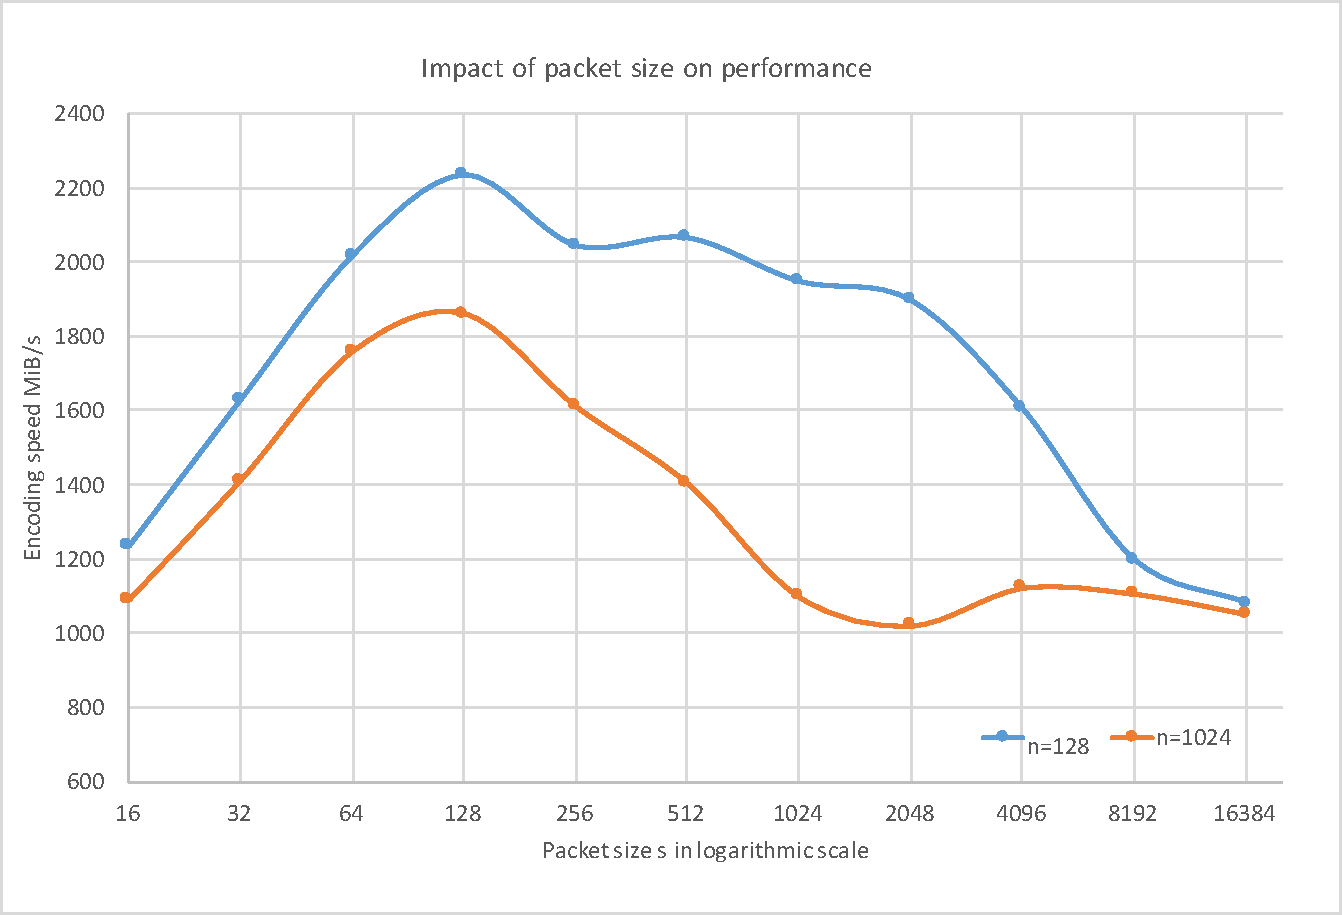
\includegraphics[width=0.7\columnwidth]{fnt_vertical_vec_pkt_size.pdf}
\caption{Vertical vectorization: impact of packet size $s$ on encoding speed of RS codes over $\gf{2^{2^4}+1}$: RS($k=8, n=128$) and RS($k=8, n=1024$).}
\label{fig:fnt_vertical_vec_pkt_size}
\end{figure}


\subsection{Impact of data length $k$}
Mindful of hyper-fragmentation, we measured the following parameters:

\begin{itemize}
\item $n \in \left\{ 256, 1024, 2048 \right\}$
\item $k \in \left\{ 8, 16, 32 \right\}$
\end{itemize}

Figure \ref{fig:fnt_k_n} shows the encoding speed for the three cases of code length $n$ over different number of data fragments $k$. Each curve represents the encoding speed for a given $n$. We observe that for each code length $n$ the speed is linear to $\frac{1}{\log{k}}$. The gap between the curves shows that the advantages of cache memory is more important for short code length than long ones. For short code length, encoding process can benefit from the different cache memories L2 and L3, while long code lengths can only exploit the L3 cache.
% * <wabernat@sonic.net> 2018-03-02T20:19:37.872Z:
% 
% Is there a unit? 
% 
% ^.
\begin{figure}[!ht]
\centering
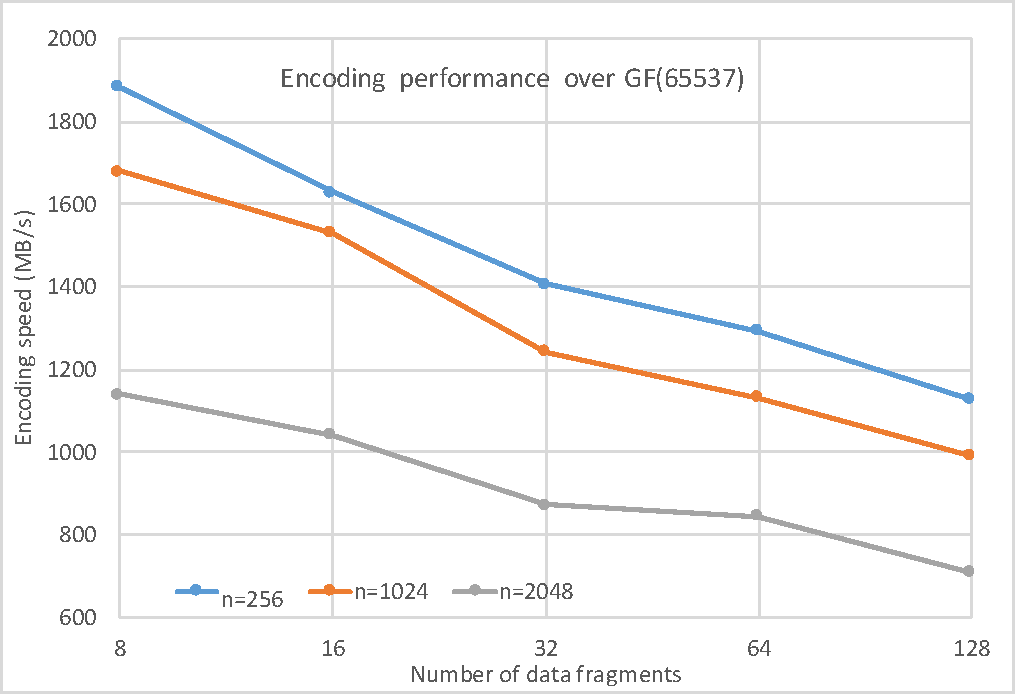
\includegraphics[width=0.7\columnwidth]{fnt_k_n.pdf}
\caption{Encoding speed of RS codes over $\gf{2^{2^4}+1}$. Each curve represents a fixed $n$.}
\label{fig:fnt_k_n}
\end{figure}

Figure \ref{fig:dec_fnt_k_n} shows the decoding speed.

\begin{figure}[!ht]
\centering
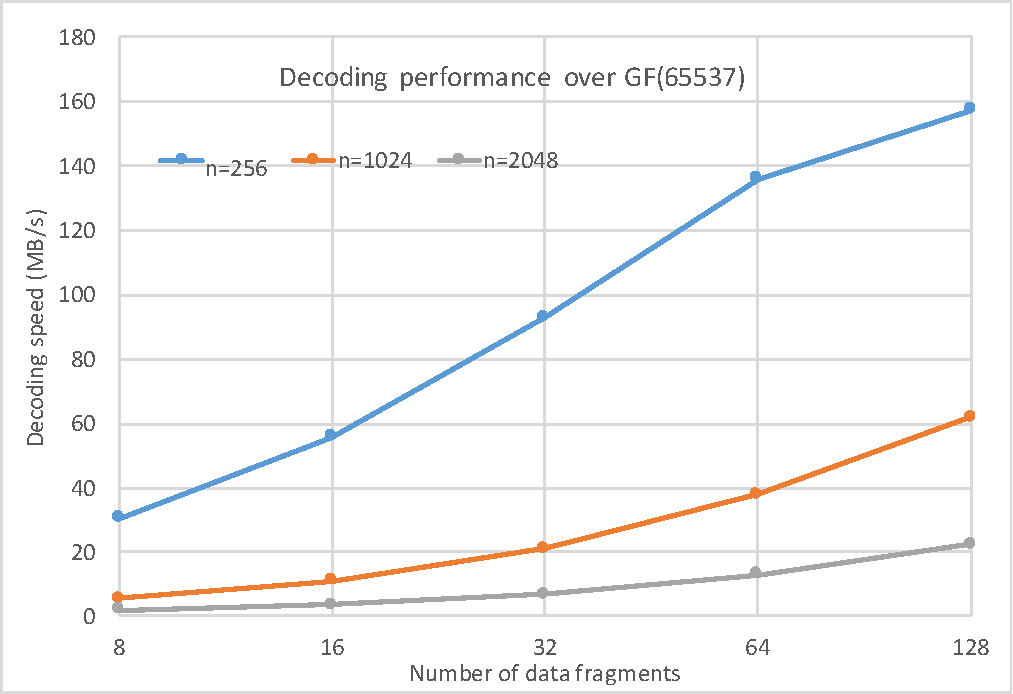
\includegraphics[width=0.7\columnwidth]{dec_fnt_k_n.pdf}
\caption{Decoding speed of RS codes over $\gf{2^{2^4}+1}$. Each curve represents a fixed $n$.}
\label{fig:dec_fnt_k_n}
\end{figure}

\section{Applications}

\subsection{Decentralized Storage over the Internet}

As drive density continues to be driven higher in keeping with Moore's Law, the price of storage continues to fall. This makes extra data copies cheaper. For example, generating and spreading hundreds of fragments from a file makes it possible to reconstruct the data while having only a fraction of the total data available. In this context, it is possible and interesting to develop a reliable decentralized cloud storage system that allows to exploit unused storage on the heterogeneous edge nodes (smartphones, laptops, servers, \dots) of the network (see figure \ref{fig:network}).

\begin{figure}[!h]
\centering
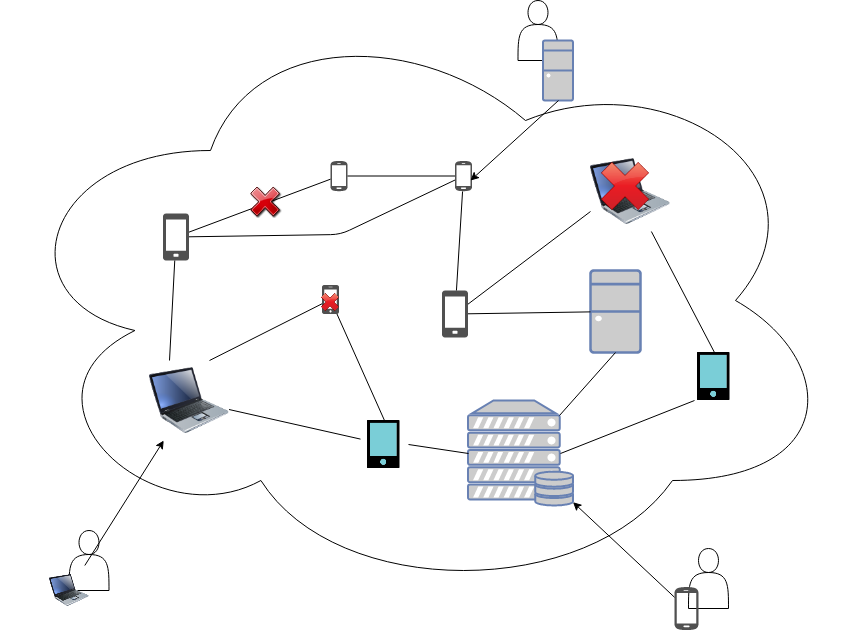
\includegraphics[width=0.7\columnwidth]{network.png}
\caption{A decentralized storage system based on heterogeneous nodes}
\label{fig:network}
\end{figure}

We have to compensate the unreliability of the underlying devices (which can go off-line anytime for any duration of time) if we want to have a reliable and resilient storage. Erasure coding is an excellent solution to increase durability while keeping the storage overhead low. Existing practical systems, such as Storj, are going toward encoding schemes like $\ec{30}{10}$, $\ec{60}{20}$ or $\ec{120}{40}$.

The systematic property is interesting but not absolutely necessary in a decentralized storage application: Indeed a decentralized storage software may choose to place the plain text data fragments on the peers having the best quality of service. But in an environment like the Internet where it is difficult to evaluate the quality of service of peers, or when the quality of service is very variable, the probability of reaching a peer that contains a plain text data fragment is getting lower as k gets bigger (see figure \ref{fig:systematic}). Therefore the systematic property becomes useless. Moreover non-systematic code are rate insensitive.

\begin{figure}[!h]
\centering
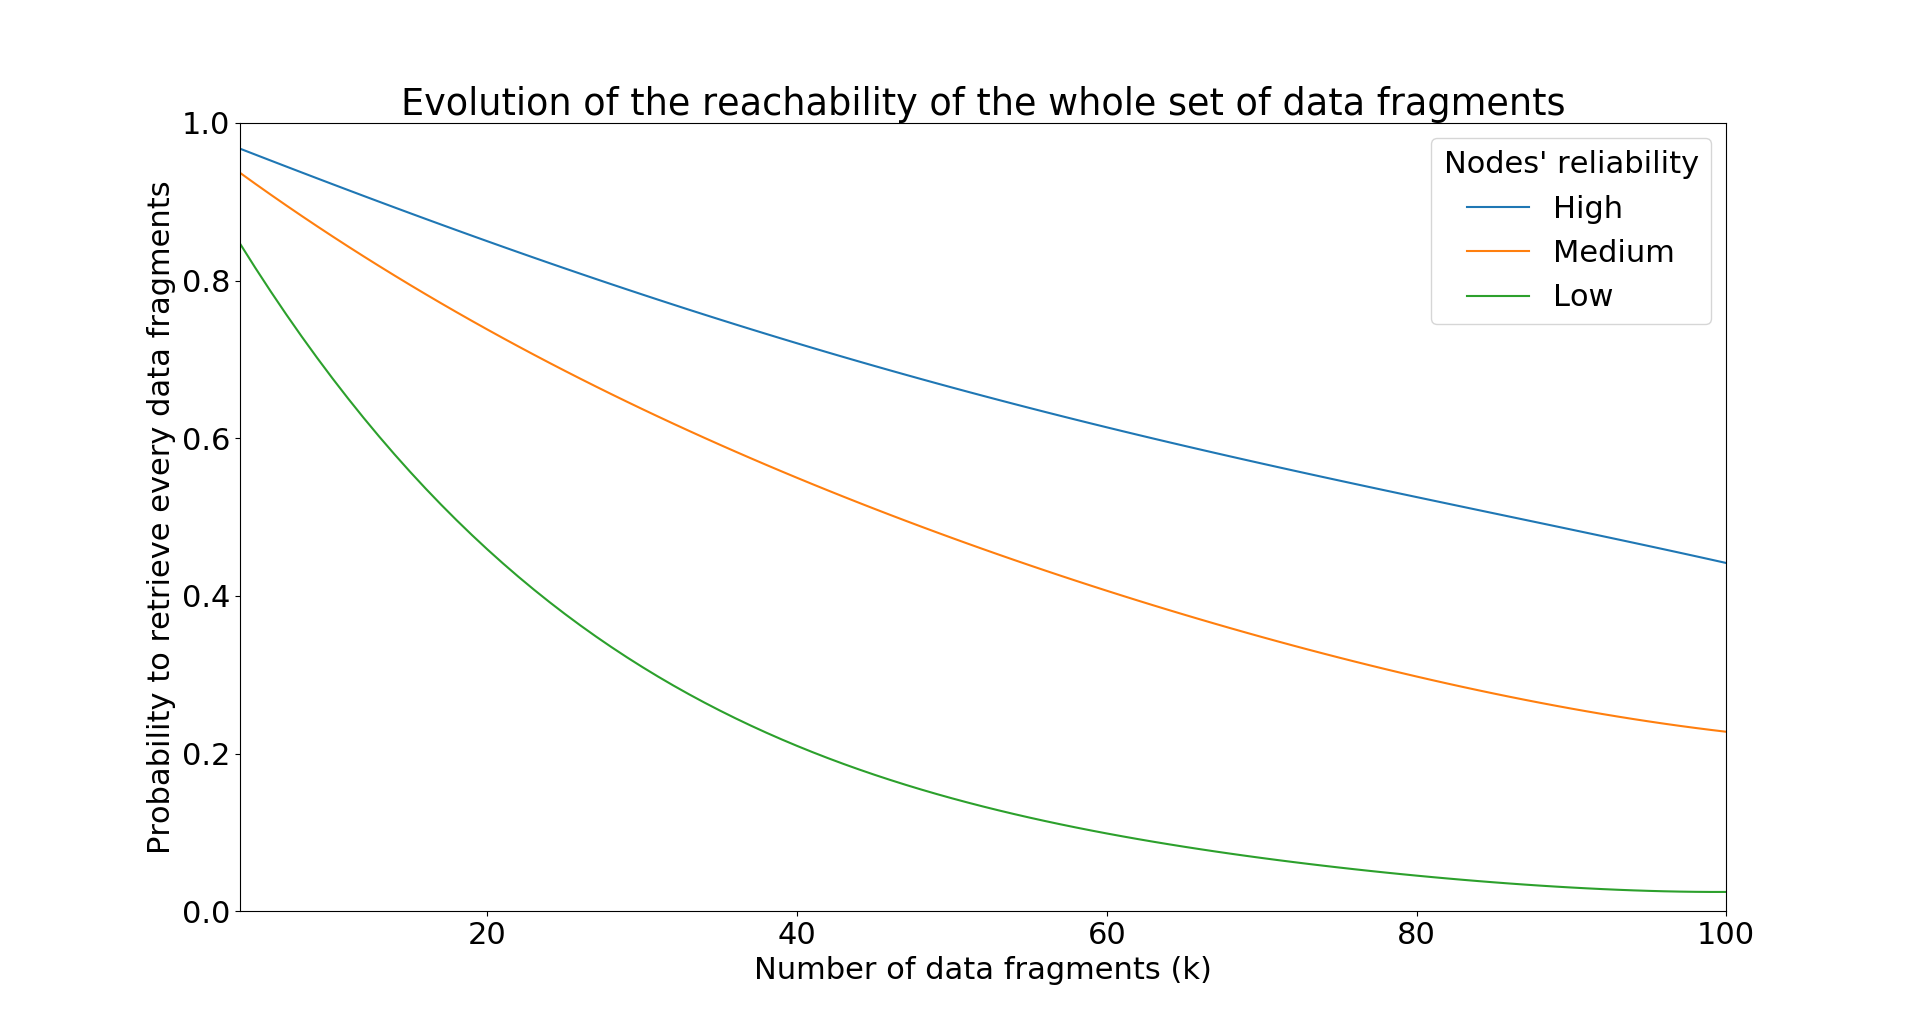
\includegraphics[width=0.7\columnwidth]{systematic.png}
\caption{Evolution of the reachability of the whole set of data fragments in function of k}
\label{fig:systematic}
\end{figure}

The adaptive rate property may also be useful in a decentralized storage application because it is not practically possible to delete and rewrite the erasure code fragments which are already in place. However if the initial durability chosen is already very high, the need for re-dimensioning the code is not critical.

The repair bandwidth is indeed a problem for RS codes but it can be mitigated in multiple ways in a decentralized storage scenario:
\begin{itemize}
\item Generally we cut a file in sub-blocks of fixed size called stripes. Since the stripes are spread in a very high number of peers, the loss of a peer will affect only one stripe with a very high probability.
\item It is possible to detect a missing fragment at the time of the read and repair it immediately after (read-repair).
\item Because of the chosen very high durability, a pro-active repair mechanism (called scrubbing) is not absolutely critical and can be scheduled rarely. 
\end{itemize}

Finally one can argue that both the systematic property and the optimization of the repair bandwidth at the level of a stripe is still advantageous in order to support get\_range() operations: the ability to read a portion of a stripe without decoding or by minimizing the decoding. The get\_range() properties might indeed be of interest in the case of a local distributed file system or a local big data cluster, but not in a decentralized storage system which targets primarily the cloud storage use case (for archival purpose) where people generally wants the files stored and retrieved in their totality.

We do compare our erasure codes with other libraries (ISA-L, Leopard, Wirehair) for k up to 1024. The ISA-L library \cite{isal} is a performance-oriented open-source library developed by Intel that implements a systematic RS code defined over $\gf{2^8}$ (which limits the code length to at most 255). Leopard \cite{leopard} is a performance-oriented RS codes using additive FFT techniques. Wirehair \cite{wirehair} is a performance-oriented hybrid LDPC library that implements a systematic code defined over $\gf{2^8}$ that also leverage SIMD instructions.

Figures \ref{fig:comp_enc_rate_1_4}, \ref{fig:comp_enc_rate_1_3}, \ref{fig:comp_enc_rate_1_2}, \ref{fig:comp_enc_rate_2_3} show encoding speeds of these codes for different coding rates 1/4, 1/3, 1/2 and 2/3 respectively. We observe that for small $k$, ISA-L codes are very good. But for $k > 24$, our codes outperform ISA-L codes thanks to FFT operations. 
%Figure \ref{fig:isal_vs_fnt_vs_leo_enc} shows encoding speeds of these codes for different number of data fragments. We observe that for small $k$, ISA-L codes are very good. But for $k > 24$, our codes outperform ISA-L codes thanks to FFT operations. 

LDPC encoding speed worsen as $k$ grows. Note the graphs shows the pure decoding speed and does not show the additional time needed to retrieve the additional fragments due to the overhead (see \cite{plank_ldpc} for a detailed study on this topic).

Wirehair is also less good for higher code rates.

Figures \ref{fig:comp_dec_rate_1_4}, \ref{fig:comp_dec_rate_1_3}, \ref{fig:comp_dec_rate_1_2}, \ref{fig:comp_dec_rate_2_3} show decoding speeds of these codes for different coding rates 1/4, 1/3, 1/2 and 2/3 respectively. We observe that average decoding time of FNT codes is about only 3.5 times longer than encoding time, compared to 8 times mentioned in \cite{fnt_lacan}. However our FNT decode speed is still slow compared to others. We plan to implement the approach defined in \cite{fnt_ida}.

\begin{figure}[!ht]
\centering
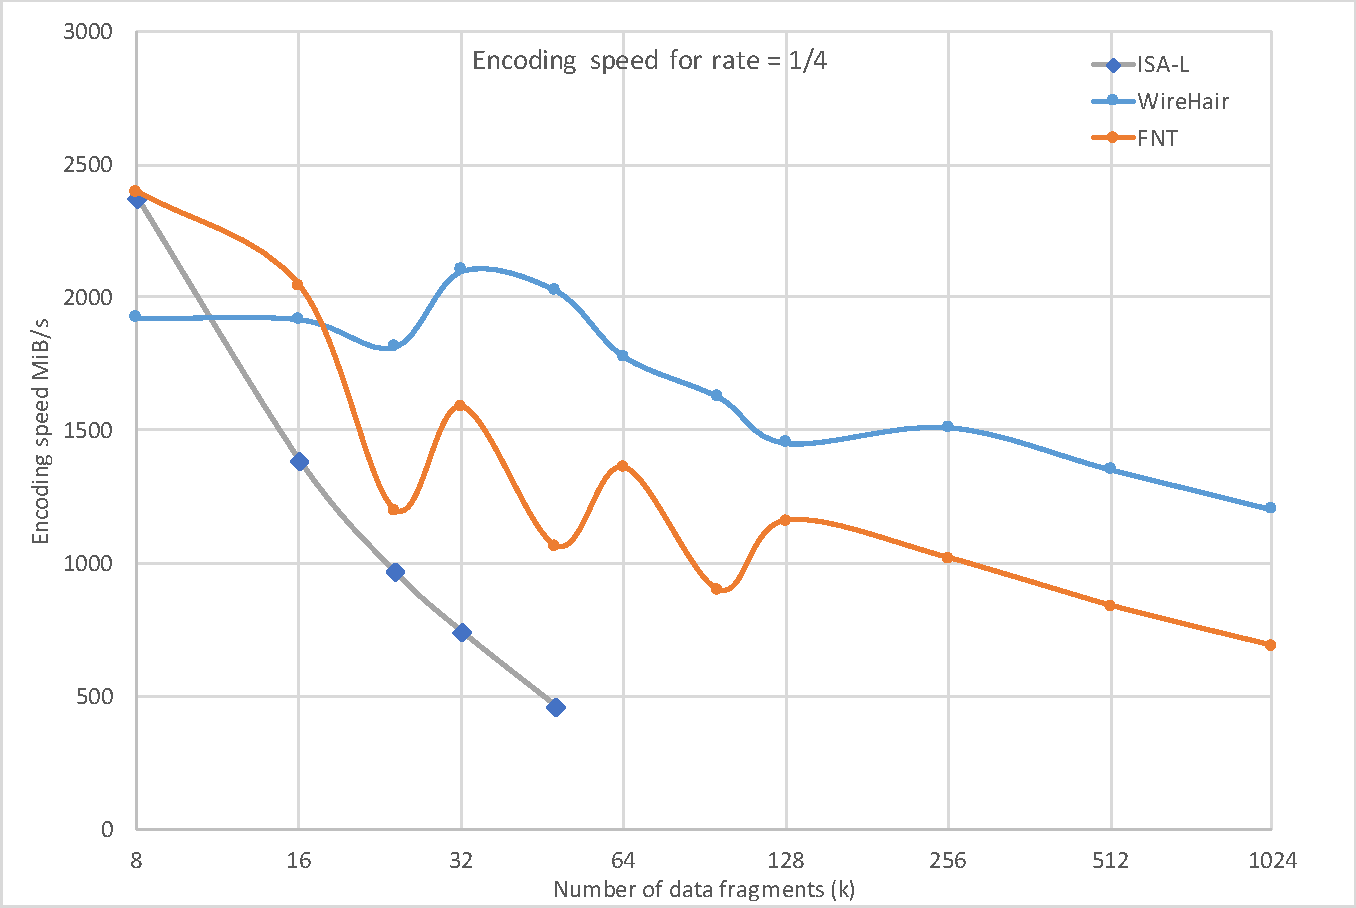
\includegraphics[width=0.7\columnwidth]{Enc_Rate1-4.pdf}
\caption{Encoding speed of RS codes of rate 1/4: comparison our FNT codes vs. ISA-L vs. Leopard vs. WireHair}
\label{fig:comp_enc_rate_1_4}
\end{figure}

\begin{figure}[!ht]
\centering
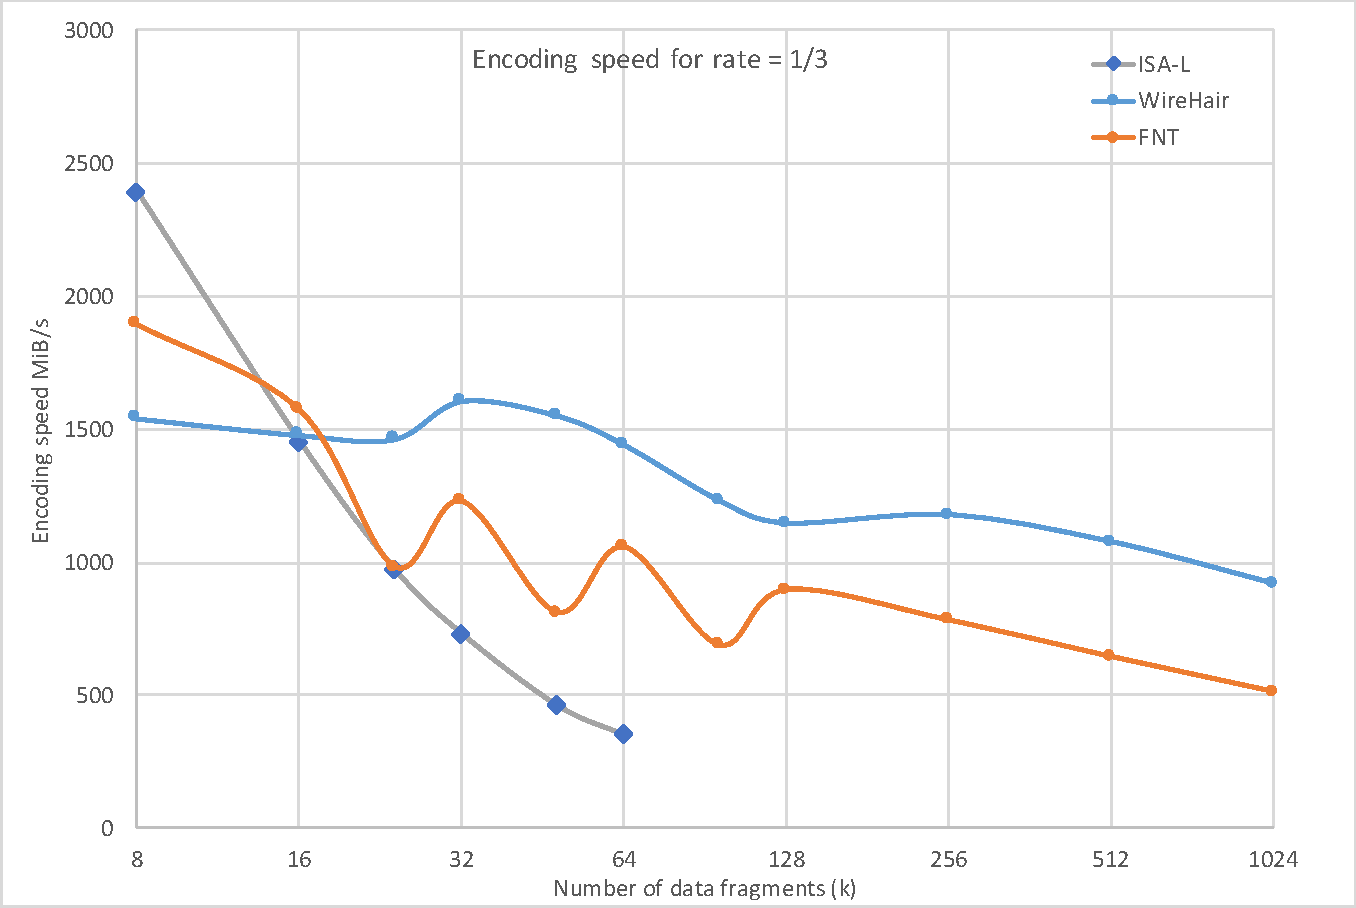
\includegraphics[width=0.7\columnwidth]{Enc_Rate1-3.pdf}
\caption{Encoding speed of RS codes of rate 1/3: comparison our FNT codes vs. ISA-L vs. Leopard vs. WireHair}
\label{fig:comp_enc_rate_1_3}
\end{figure}

\begin{figure}[!ht]
\centering
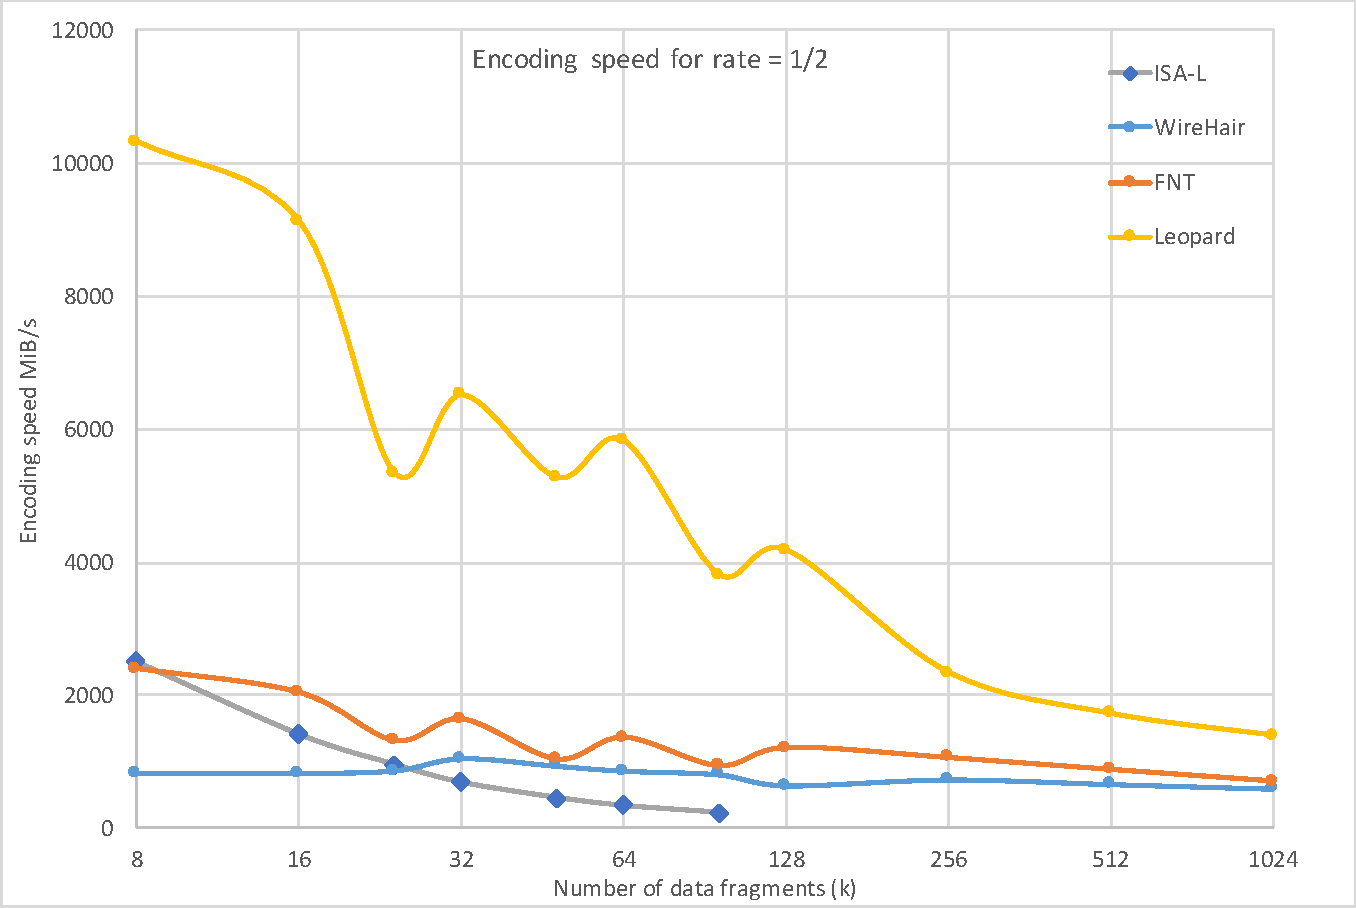
\includegraphics[width=0.7\columnwidth]{Enc_Rate1-2.pdf}
\caption{Encoding speed of RS codes of rate 1/2: comparison our FNT codes vs. ISA-L vs. Leopard vs. WireHair}
\label{fig:comp_enc_rate_1_2}
\end{figure}

\begin{figure}[!ht]
\centering
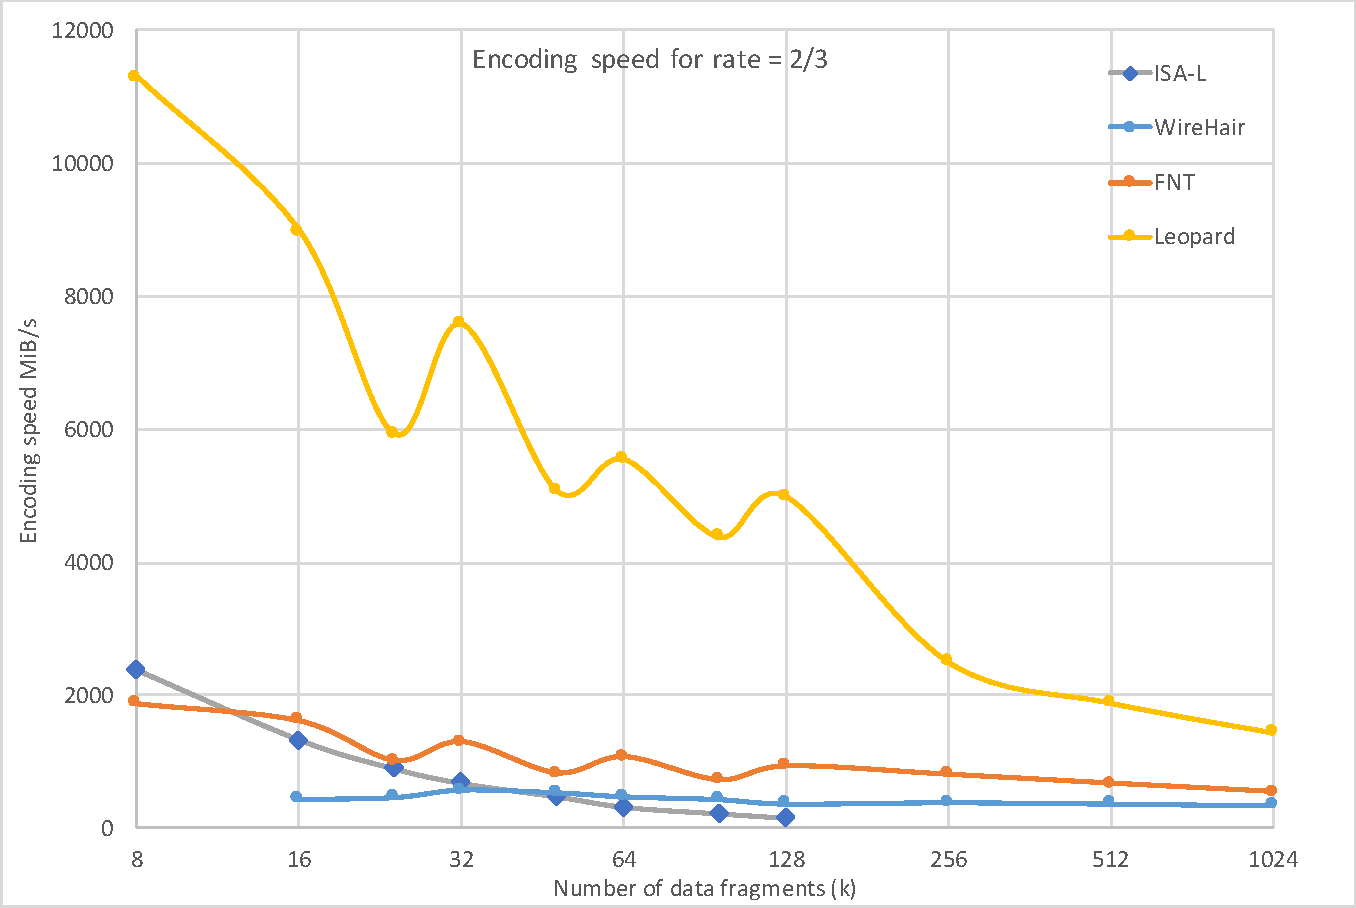
\includegraphics[width=0.7\columnwidth]{Enc_Rate2-3.pdf}
\caption{Encoding speed of RS codes of rate 2/3: comparison our FNT codes vs. ISA-L vs. Leopard vs. WireHair}
\label{fig:comp_enc_rate_2_3}
\end{figure}

\begin{figure}[!ht]
\centering
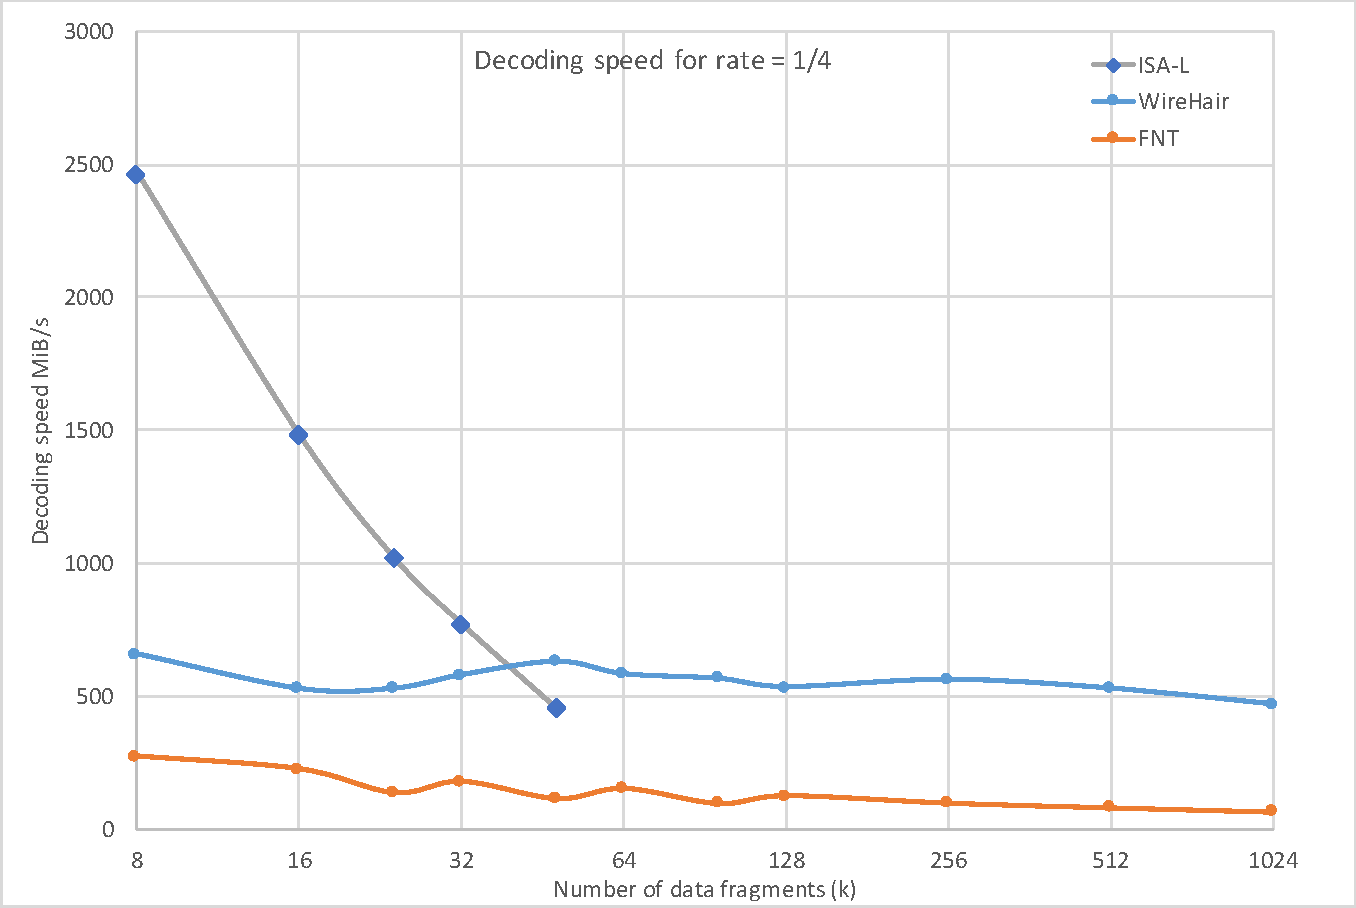
\includegraphics[width=0.7\columnwidth]{Dec_Rate1-4.pdf}
\caption{Decoding speed of RS codes of rate 1/4: comparison our FNT codes vs. ISA-L vs. Leopard vs. WireHair}
\label{fig:comp_dec_rate_1_4}
\end{figure}

\begin{figure}[!ht]
\centering
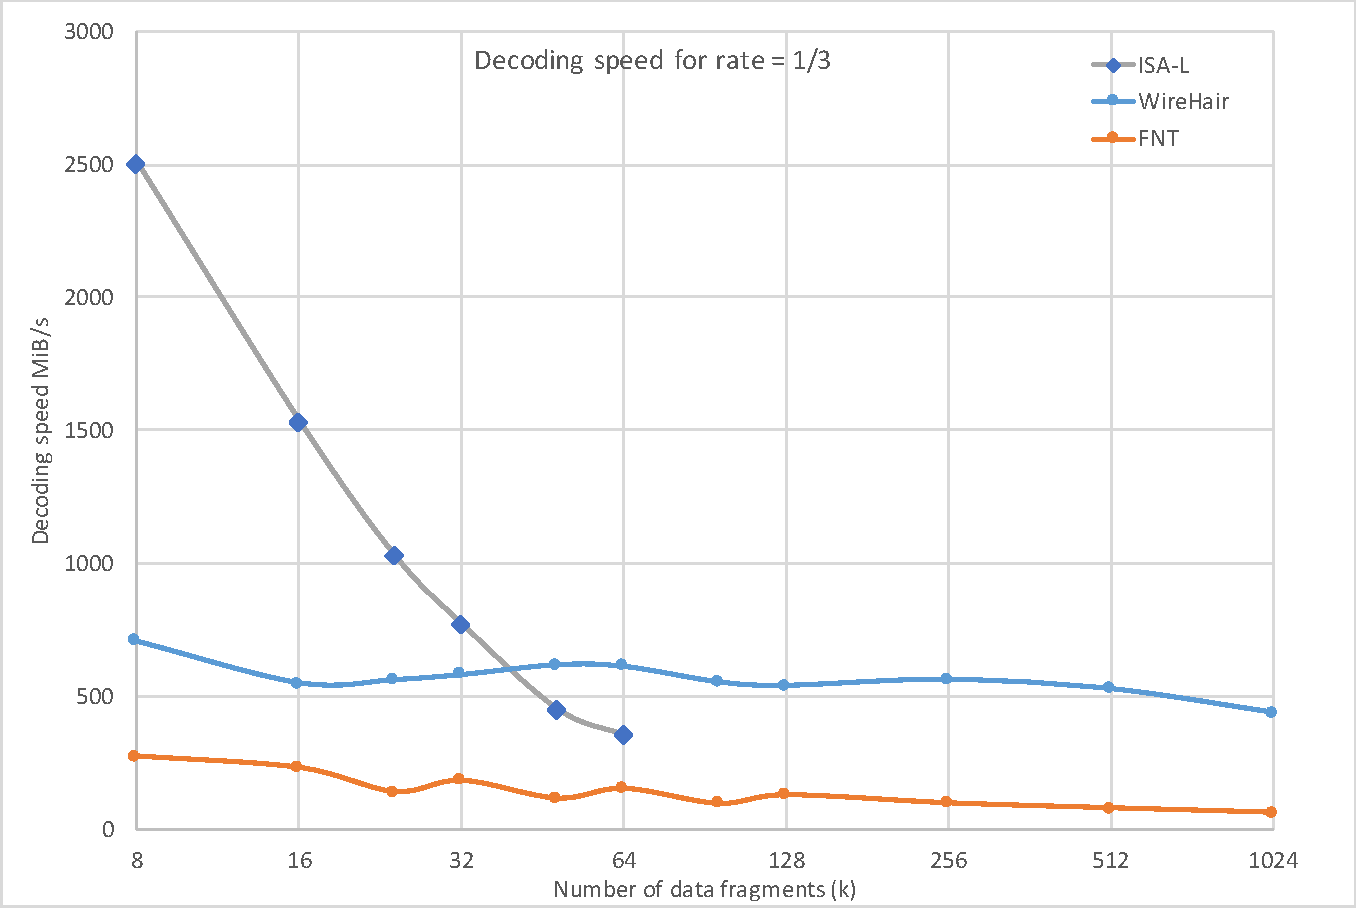
\includegraphics[width=0.7\columnwidth]{Dec_Rate1-3.pdf}
\caption{Decoding speed of RS codes of rate 1/3: comparison our FNT codes vs. ISA-L vs. Leopard vs. WireHair}
\label{fig:comp_dec_rate_1_3}
\end{figure}

\begin{figure}[!ht]
\centering
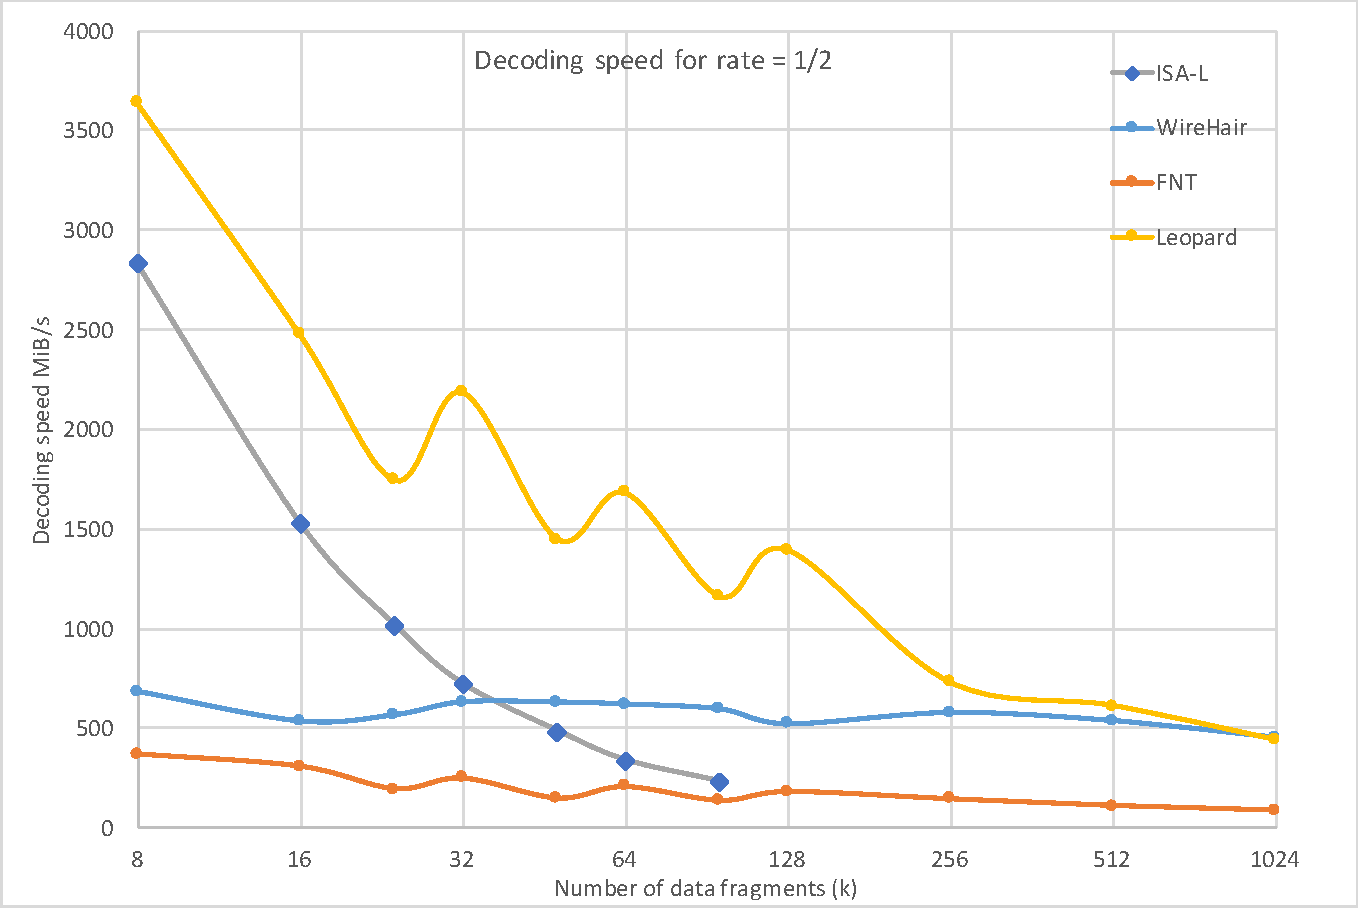
\includegraphics[width=0.7\columnwidth]{Dec_Rate1-2.pdf}
\caption{Decoding speed of RS codes of rate 1/2: comparison our FNT codes vs. ISA-L vs. Leopard vs. WireHair}
\label{fig:comp_dec_rate_1_2}
\end{figure}

\begin{figure}[!ht]
\centering
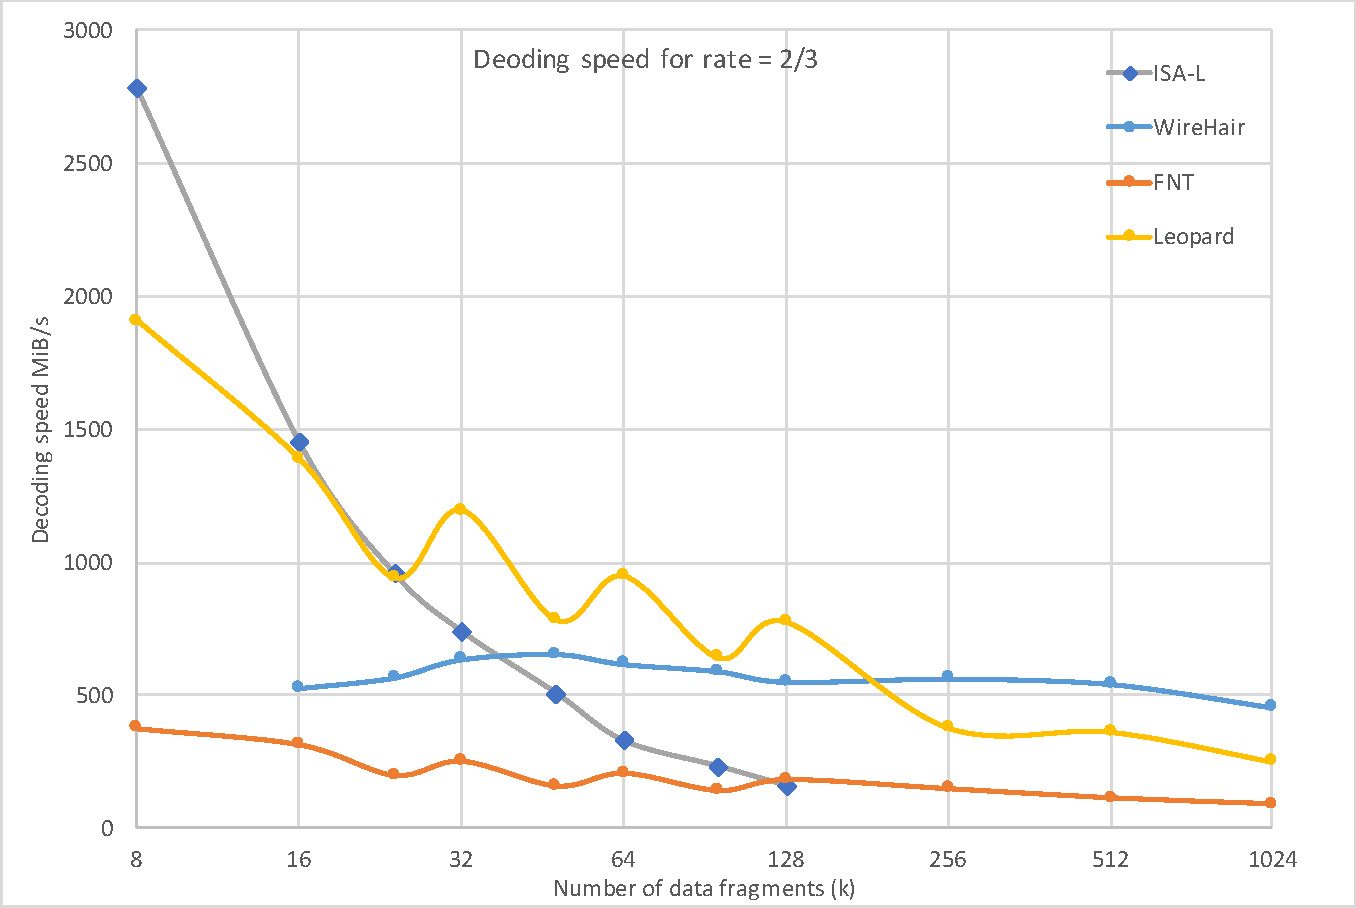
\includegraphics[width=0.7\columnwidth]{Dec_Rate2-3.pdf}
\caption{Decoding speed of RS codes of rate 2/3: comparison our FNT codes vs. ISA-L vs. Leopard vs. WireHair}
\label{fig:comp_dec_rate_2_3}
\end{figure}

As wee see in practical decentralized storage applications like Storj the typical code rate is 1/3 or 1/4 which means relatively high durability and relatively low number of fragments to retrieve which is good for latency. LDPC such as Wirehair show to be very good, although non MDS, we show that FNT has a relatively good performance but is still inferior to LDPC, we think we can improve FNT perf in improving the FFT method (we currently implement a bit-reverse method that requires copying data and we could replace by other more efficient methods). We also think that accelerating additive FFT such as what has been done in Leopard \cite{leopard} is very promising.]

Another interesting property for this application is the confidentiality of the erasure code, even though the client decides to encrypt or not the files beforehand, using a non-systematic FNT augments the security.

\subsection{Real-Time Video Encoding High-Quality Streaming}

There are many types of video streams. For high quality ingress of a broadcast system, the master stream is typically broken up into pieces and encoded to lower quality with a few seconds of delay.

Those real-time video high quality streams with 30\% interleaving (code rate 2/3) have many pieces, and are generally encoded using $\bigo{N^2}$ streaming convolutional codes e.g. like CauchyCaterpillar \cite{cauchycaterpillar} which operates on  $\gf{2^8}$ and is limited to 2MB/s. To go faster the technique generally used is interleaving block codes (which is how video FEC is usually done \cite{al_fec}). The overhead from using something fast like a XOR based LDPC on $\gf{2^2}$ is highly inefficient. Our MDS NTT approach is much better because we have no overhead and we can keep up with the speed.

In this type of application there is a need for a systematic code. As wee see in \cite{leopard}, \cite{fft_add_chung} and \cite{fnt_lacan} we can implement systematic NTT based codes with lesser but similar performance.

\section{Conclusion}

NTT codes offer superior encoding performance compared to matrix-based RS erasure codes for applications requiring $n \gtrapprox 24$ symbols, and are simpler than LDPC codes, while supporting all the desirable properties: Fast, MDS, systematic or non-systematic, confidential (for systematic codes). As we have seen the optimization of repair bandwidth as offered by LRC codes is not critical for a decentralized cloud storage application. The most important property for us remains the MDS property as a rock solid contract: being sure than if k fragments are available then the data is recoverable. Also, as we seen, FNT aka multiplicative FFT codes offer not necessarily always faster but more predictive performance than additive FFT codes for various $n$. 

Those codes may have other potential applications such as high-quality video streaming but a lot of experiments and analysis have yet to be conducted.

\section{Future Work}
The next steps for the QuadIron library are in order of priority:
\begin{itemize}
\item Optimize the multiplicative FFT decoding, which is for now relatively slow (\cite{fnt_ida} and \cite{gao_decode} has shown a way to optimize). It can be possible for special values of k and m, e.g. $k \% m = 0$ or $m \% k = 0$.
\item Optimize additive FFTs (for now we don't have any HW acceleration).
\item Implement additive FFT based systematic codes.
\item Design and implement NTT based adaptive codes for multiplicative FFTs.
\item Design and implement NTT based adaptive codes for additive FFTs.
\item Implement Frobenius multiplicative FFT \cite{frobenius_fft}.
\item Implement Frobenius additive FFT \cite{frob_additive}.
\end{itemize}

\bibliographystyle{unsrt}
\bibliography{bib}


\section*{Authors}

\begin{description}

\item[Vianney Rancurel] is a computer professional with more than 20 years of experience designing and developing computer products. He currently leads the Scality research team which is responsible for feasibility studies, prototypes and patents/publications. Previously he worked in the messaging and telco industries on both software and hardware technologies at Bizanga, Borea Technologies, and Freescale. He was also a professor at the EPITA engineering school and was responsible for its System Research Lab. His specialties are system software programming, distributed systems, embedded systems and security. Vianney has a degree of Systems \& Networks Engineering from EPITA.

% if you will not have a photo at all:
\item[Lam Pham-Sy] is a research engineer working on information theory and computer science. His main research focuses on different families of forward erasure correcting codes such as Reed-Solomon codes, Low-Density Parity-Check codes, Locally Repairable codes etc. Their application covers from digital communication to data storage. He did his PhD program in a collaboration between CEA-Leti and Eutelsat S.A. on the subject of forward erasure codes for satellite communications. Afterwards, he continued his researches at ETIS laboratory and at Orange Labs. Currently he works at Scality S.A. as a research engineer whose research topics include application of erasure codes in distributed storage systems, finite field arithmetics.

\item[Sylvain Laperche] is a code craftsman. With a background in biotech engineering,he learnt how to hack bacteria before learning how to hack a computer. That changed when it studied bioinformatics, and since then he honed and applied its skill on a wide set of problematics: genome sequencing, complex embedded systems, climate modelling at European scale, mass-scale geolocation for telco industries. Its steps led him to work on distributed storage systems and he currently works as an R\&D engineer at Scality.
Sylvain Laperche has an Engineer's degree in Hardware, Circuit Design and Embedded Systems from ISIMA.

\end{description}

\end{document}


